TODO: where should this go? Titled ``Secondary fan example''
\begin{center}
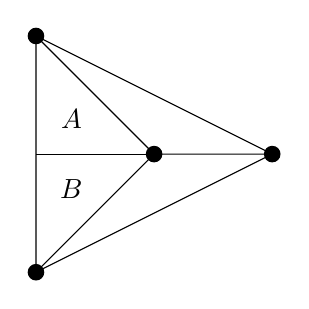
\begin{tikzpicture}[scale=1.5]
    % Define the points for easier reference
    \coordinate (A) at (1,0);
    \coordinate (B) at (2,0);
    \coordinate (C) at (0,1);
    \coordinate (D) at (0,-1);
    \coordinate (E) at (0,0);
    \coordinate (F) at (1.2,0.2);
    \coordinate (G) at (2.2,0.2);
    \coordinate (H) at (0.2,1.2);
    \coordinate (I) at (0.2,-.8);
    \coordinate (J) at (0.2,0.2);

    % Draw all line segments connecting the points
    \draw (A) -- (B) -- (C) -- cycle;
    \draw (A) -- (D) -- (C);
    \draw (B) -- (D); 
    \draw (A) -- (E);

    % Plot the points (as small black circles)
    \fill (A) circle (2pt);
    \fill (B) circle (2pt);
    \fill (C) circle (2pt);
    \fill (D) circle (2pt);
    \draw (.3,.3) node {$A$};
    \draw (.3,-.3) node {$B$};
\end{tikzpicture}
\end{center}

\subsection{TODO: July 23rd}

\begin{itemize}
\item Daniel and Michael: Sections 1-5.

\item  David: Suggests moving the blurb at the begining of 7 to someplace near the beginning of the notes, and referring back to it. \michael{Agreed. In fact, all of that content is already introduced in lecture 4, so I just commented out that paragraph.}
\item David:** Says `$M_L$` is poor notation because `M` already has a central role.\michael{Agree with this too. I will leave it to David/Jay to make this edit.}
\item David: Sections 6-9. -- reference needed before 8.5 ( I left the \david{where?} macro in the tex file.) \michael{Added.}
In section 6 just before Demazure Vanishing michael asked:
%\michael{This is (close to) \cite{BBB+24}*{Lemma 2.20}, which isn't that easy, right?}
\michael{that comment of mine can be ignored.}

\item Michael: Section 12-16.
\item Lauren: Section 11 and Appendix A.

\item Jay: Package to be able to: and package on a website and ready to roll.
  \begin{enumerate}
  \item Compute HHL resolutions.
  \item Compute the Bondal-Thomsen collection.
  \item Compute the secondary fan.
  \item Compute Fourier-Mukai transform of line bundles.
  \item BGG and Tate resolutions (but just leveraging what already exists).
  \end{enumerate}

\item Mahrud: Appendix C. Appendix should cover each of these for the Hirzebruch surface of type 3 as follows:
  \begin{enumerate}
  \item HHL resolution of diagonal $X \subseteq X \times X$
  \item HHL resolution of point in X
  \item BT collection of Hirzebruch surface of type 3.
  \item FM trasnform of every line bundle in Theta for Hirzebruch of type 3 and for the corresponding PP(1,1,3)
  \item Secondary fan of Hirz of type 3.
  \end{enumerate}
  Examples should involve both Macaulay2 code and clear TeX writeup with diagrams when relevant.

\item Everyone: feel free to add comments in any section, but please be avoid directly editing unassigned sections at this point.
  Jay: Add a few things to Sections 8 and 9 by end of day Friday.
\item Everyone:  feedback on Section 7 (also on Section 6, though it’s been gone over a few times).
\item Lectures 10, 17-19 are in pretty good shape it seems.  Comments welcome, but lower priority than the rest.
\item Sections 12-16: higher priority for comments.
\end{itemize}

\subsection{Wish List (pre-NH)}
\begin{enumerate}
\item  Add a simple proof that the free module degrees in BCHSY come from Bondal-Thomsen.
\item  Mention that BCHSY works in the radical case and include an example (maybe an example where the defining ideal of $X\subseteq Y$ is radical but not prime, e.g. the case of a point in a fake projective plane, which appeared in Brown-Erman's paper.)
\item
\end{enumerate}

\subsection{Work on Notes and an M2 package for the week of July 13}
Notes:
\begin{itemize}
\item Main focus for DE, JY, MS, LCH: 5-8, 10 need a lot of work then expand on 1-4
\item The BCHSY treatment of HHL res should be broken into 3 lectures (sect 6-8) (possible outline at head of sect 6)
\item comments only on 11-14 (except for Michael)
\item Lauren should be chief of the material on the secondary fan
\item DE will work on Achinger material --  in sect 5
\item Lectures 1-5 could use some significant fleshing out, especially if we want this to eventually be a standalone document.
\end{itemize}

M2 Package
\begin{itemize}
\item  Have the package for computing HHL resolutions of equivariant sheaves and toric subvarietes in good enough shape, including documentation, to share with all participants.
\item BT monads in M2?
\item  Include code for computing the secondary fan associated to a multigraded ring.
\item  Can we write code that would allow for Fourier-Mukai transforms of line bundles, as in the Transform Lemma?
\end{itemize}
